\section{Controlled Numerical Validation}
\label{sec:numerical-validation}

The main results are analytic.  This section tests the computational identities
and certificates on deterministic synthetic instances, with no learned model
or external data.  In orthonormal action coordinates we set
\[
  A=\begin{pmatrix}I_m\\0\\0\end{pmatrix},\qquad
  B=\begin{pmatrix}M\\N_a\\0\end{pmatrix},\qquad M\succ0,
\]
where \(N_a\in\mathbb R^{s\times m}\), so the active dimension is
\(r=m+s\).  The generator forms \(R_0\), \(\rho\), and both residuals from
the formulas in \cref{sec:action-bundle,eq:active-residual-splitting}.  Matrix
roots, logarithms, and exponentials use symmetric eigendecompositions.  All
reported distributions use the fixed seeds \(7,19,43\); the complete
configuration and raw results accompany the source.

\paragraph{Certificates and exact active realization.}
For \(d=24\), \(m=s=4\), we computed a reference solution to residual
\(10^{-13}\), then ran both the full and active iterations from the identity
until the full residual was at most \(10^{-5}\).  Across all recorded iterates,
the largest ratios
\[
  \frac{\dai(\Sigma_k,\Sigma_\star)}{\fro{W_B(\Sigma_k)}}
  \quad\text{and}\quad
  \frac{f_B(\Sigma_k)-f_B(\Sigma_\star)}
       {\tfrac12\fro{W_B(\Sigma_k)}^2}
\]
were \(0.972\) and \(0.971\), respectively, consistent with
\cref{eq:solver-distance-certificate,eq:solver-gap-certificate}.  The maximum
ratios are conservative: the reference certificate contributes \(10^{-13}\)
to the numerator of the distance ratio and at most \(5\times10^{-27}\) to the
objective-gap numerator.  The maximum
relative difference between the reconstructed active iterate and the full
iterate was \(2.1\times10^{-15}\).  Relative action infeasibility stayed below
\(1.1\times10^{-16}\), and absolute log-determinant drift below
\(1.8\times10^{-14}\).  These last quantities measure floating-point drift;
they are not interval certificates.

\begin{figure}[t]
  \centering
  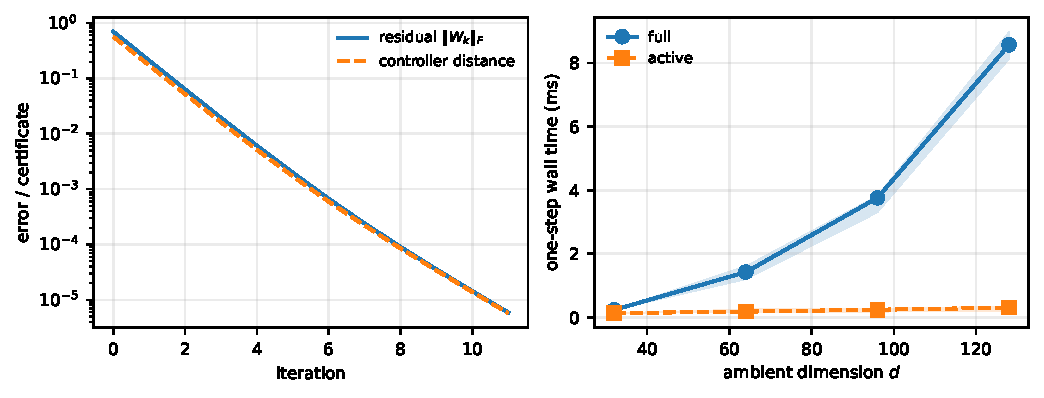
\includegraphics[width=0.94\textwidth]{figures/validation.pdf}
  \caption{Left: residual certificate and reference controller distance for one
  fixed synthetic instance; the other seeds give the same qualitative decay.
  Right: median wall time for one full and active step, with interquartile
  bands over three seeds and seven repetitions after an unmeasured warm-up;
  measurement order is alternated and BLAS uses one thread.  Here \(m=s=4\), so the active
  spectral kernel remains \(r=8\) while \(d\) grows.  Timings are
  implementation and hardware dependent; the invariant result is the kernel
  dimension in \cref{cor:active-core-solver}.}
  \label{fig:validation}
\end{figure}

\paragraph{Dimension and boundary sensitivity.}
We fixed \(m=s=4\) and used ambient dimensions \(32,64,96,128\).  The full
step acts on a dense matrix whose order grows with \(d\), whereas the active
step keeps an order-eight spectral kernel.  At \(d=128\), the observed median one-step times
were \(8.57\) ms and \(0.307\) ms.  The median of the \(21\) paired full/active
time ratios was \(26.9\) in this reference Python implementation.  The
corresponding storage proxies \(d^2\) and
\(dm+r^2\) are \(16384\) and \(576\) scalar entries.

To approach the feasibility boundary, we varied
\(\lambda_{\min}(A^\top B)=\lambda_{\min}(M)\) from \(1\) to \(10^{-3}\)
while holding dimensions and random directions fixed.  Median \(D_0\) grew
from \(0.994\) to \(13.98\), median \(L_0\) from \(1.159\) to \(9.885\), and
the median iterations needed for residual \(10^{-8}\) from \(8\) to \(126\)
(the range over all instances was \(8\)--\(143\)).  Thus the experiment
exposes the rate constant's sensitivity before feasibility is lost; it does
not extrapolate the theorem to singular \(A^\top B\).

\paragraph{Same-objective baseline and nested recovery.}
We also compared the explicit \(1/L_0\) step with a Riemannian gradient method
using Armijo backtracking on the same hidden-coordinate objective and from the
same identity start.  At residual tolerance \(10^{-8}\), median iteration
counts over the three seeds were \(17\) and \(11\), while median objective
evaluations were \(18\) and \(23\), respectively.  Thus line search used fewer
accepted steps but more objective evaluations; the explicit step supplies its
rate and admissibility without backtracking.  This comparison isolates step
selection and does not compare against methods with different feasible models.

Finally, for random \(8\times8\) Hessians we used cumulative ranks
\(2,4,7\) and stopped each inner projection at residual \(10^{-3}\).  Across
three seeds, the largest actual-inner-error/certificate ratio was \(0.983\),
and the largest left/right ratio in
\cref{eq:approximate-multisecant-pythagorean} was
\(1+9.3\times10^{-15}\).  The rank-seven output recovered \(P_\star\) within
\(1.3\times10^{-14}\) AIRM distance; relative cumulative-action error stayed
below \(2.4\times10^{-15}\).  This test evaluates the exact-feasibility model
in floating point and reports the resulting feasibility drift separately.

\begin{figure}[t]
  \centering
  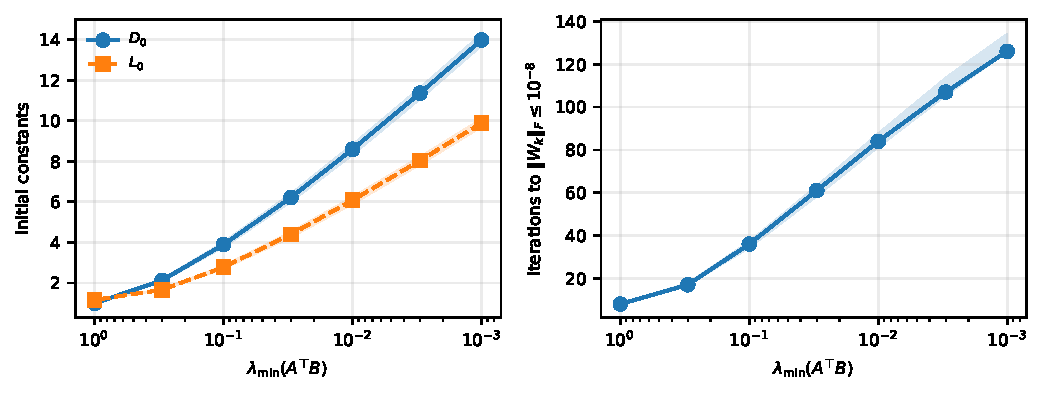
\includegraphics[width=0.94\textwidth]{figures/boundary_sensitivity.pdf}
  \caption{Sensitivity as \(A^\top B\) approaches the positive-definite
  boundary.  Curves show medians and shaded interquartile ranges over the three
  fixed seeds.  Both the analytic radius majorant and the observed iteration
  count deteriorate while every tested instance remains feasible.}
  \label{fig:boundary-sensitivity}
\end{figure}

These experiments test the exact formulas in standard floating point.  They
do not instantiate the certified residual-oracle model of
\cref{cor:inexact-action-solver}; an end-to-end implementation of that model
would require rigorous enclosures for every matrix function and update.
